\chapter{Cài đặt và xây dựng hệ thống}
\label{chap:cai_dat}

Chương này mô tả cách các thành phần thiết kế ở Chương~\ref{chap:thiet_ke} được cài đặt, và những giới hạn còn lại khi triển khai.

\section{Môi trường cài đặt}
\label{sec:moi-truong}

Bảng~\ref{tab:c4_moitruong} liệt kê môi trường của máy phát triển, có GPU Quadro T2000 4~GB, dùng để lập chỉ mục, đo độ trễ và chạy bản trình diễn. Ba bản trọng số tinh chỉnh được huấn luyện trên máy khác (Mục~\ref{sec:tinh-chinh}).

\begin{table}[H]
\centering
\caption{Môi trường cài đặt trên máy phát triển}
\label{tab:c4_moitruong}
\small
\renewcommand{\arraystretch}{1.15}
\begin{tabularx}{\textwidth}{@{}p{4.5cm} p{3.7cm} X@{}}
\toprule
\textbf{Thành phần} & \textbf{Phiên bản} & \textbf{Vai trò} \\
\midrule
GPU & Quadro T2000, 4~GB & Lập chỉ mục và mã hoá truy vấn \\
PyTorch & 2.5.1 (CUDA 12.1) & Suy luận trên máy phát triển \\
Transformers~\cite{wolf2020transformers} & 4.57.6 & Nạp SigLIP 2, SigLIP 1 và ViSigLIP-OT \\
PEFT~\cite{mangrulkar2022peft} & 0.20.0 & Tham số bổ sung (adapter) LoRA và DoRA \\
sentence-transformers~\cite{reimers2019sbert} & 5.1.0 & Nạp CLIP \\
rank-bm25~\cite{brown2020rankbm25} & 0.2.2 & Phương pháp đối chứng BM25 \\
Qdrant~\cite{qdrantdocs}, máy chủ và máy khách & 1.19.0 & Kho vector của bản trình diễn \\
\bottomrule
\end{tabularx}
\end{table}

\section{Nạp và chuẩn hoá dữ liệu}
\label{sec:nap-du-lieu}

Dữ liệu lấy từ Fashionpedia~\cite{jia2020fashionpedia}, bản sao trên Hugging Face, gồm 45.623 ảnh huấn luyện và 1.158 ảnh xác thực, tổng cộng 46.781 ảnh. Bản này chỉ có danh mục và hộp bao, không có màu hay chất liệu. Khi nạp, nhóm tính mã băm cảm nhận (pHash) của từng ảnh và loại 365 ảnh trùng hoặc không đọc được, còn 46.416 sản phẩm (số liệu hiện có không tách riêng hai lý do). Việc loại trùng diễn ra trước khi chia, nên hai ảnh giống hệt nhau không thể nằm ở hai tập khác nhau. Các sản phẩm còn lại được chia ngẫu nhiên theo tỷ lệ 70/15/15, với seed 42. Ảnh gần trùng, chẳng hạn cùng một sản phẩm chụp lại, có mã băm khác nên không bị loại. Nhóm chưa kiểm tra các ảnh gần trùng này, vì vậy tập kiểm tra có thể chứa ảnh gần giống ảnh huấn luyện.

Bảng~\ref{tab:c4_chia} cho thấy kết quả chia. Kho sản phẩm dùng để đánh giá và trình diễn là tập kiểm tra gồm 6.963 ảnh, chưa xuất hiện trong quá trình tinh chỉnh.

\begin{table}[H]
\centering
\caption{Ba tập dữ liệu sau khi lọc trùng và chia}
\label{tab:c4_chia}
\small
\renewcommand{\arraystretch}{1.15}
\begin{tabularx}{\textwidth}{@{}p{3.0cm} r@{\hspace{1.5em}}X@{}}
\toprule
\textbf{Tập} & \textbf{Số sản phẩm} & \textbf{Vai trò} \\
\midrule
Huấn luyện & 32.491 & Tinh chỉnh adapter \\
Xác thực & 6.962 & Chọn epoch tốt nhất \\
Kiểm tra & 6.963 & Kho sản phẩm được lập chỉ mục, đánh giá và trình diễn \\
\bottomrule
\end{tabularx}
\end{table}

Mỗi sản phẩm là một ảnh người mặc cả bộ trang phục. Tên sản phẩm liệt kê mọi món có trong ảnh (trung bình 2,95 món, nhiều nhất 11 món), còn trường danh mục chỉ ghi món đầu tiên. Trường danh mục dùng 46 loại của Fashionpedia, đã dịch tên sang tiếng Việt: 13 trang phục chính, 14 phụ kiện và 19 bộ phận hay chi tiết. Văn bản dùng để lập chỉ mục và cho BM25 chỉ gồm tên các danh mục, đã chuẩn hoá Unicode NFC và đưa về chữ thường, giữ nguyên dấu. Chú thích huấn luyện (caption) của mỗi ảnh gồm tên tiếng Việt của mọi danh mục trong ảnh, danh mục chính và tên các chi tiết bộ phận; không có màu, chất liệu hay giá.

\section{Bộ mã hoá ảnh và văn bản}
\label{sec:ma-hoa}

Mọi hệ tìm kiếm bằng vector dùng chung một giao diện mã hoá: nhận danh sách văn bản hoặc ảnh, trả về vector đã chuẩn hoá độ dài. Nhờ vậy muốn đổi mô hình chỉ cần sửa tệp cấu hình, phần còn lại của hệ thống giữ nguyên (Mục~\ref{sec:kien-truc}). Bảng~\ref{tab:c4_mahoa} tóm tắt các bộ mã hoá đã cài đặt (dòng cuối là bộ mã hoá mô phỏng, dùng khi kiểm thử và chạy cấu hình mặc định).

\begin{table}[H]
\centering
\caption{Các bộ mã hoá đã cài đặt}
\label{tab:c4_mahoa}
\small
\renewcommand{\arraystretch}{1.15}
\begin{tabularx}{\textwidth}{@{}p{3.6cm} r p{3.0cm} X@{}}
\toprule
\textbf{Bộ mã hoá} & \textbf{Số chiều} & \textbf{Giới hạn văn bản} & \textbf{Ghi chú} \\
\midrule
SigLIP 2~\cite{tschannen2025siglip2} & 768 & Đệm đến 64 token & Mô hình chính; mặc định chạy bf16 \\
CLIP ViT-B/32~\cite{radford2021clip} & 512 & 77 token & Đối chứng zero-shot \\
ViSigLIP-OT~\cite{viclipot2026} & 768 & Theo mô hình & Chạy trên CPU vì vector ảnh ra giá trị NaN trên GPU \\
SigLIP 1~\cite{zhai2023siglip} & 768 & Đệm đến 64 token & Ảnh đầu vào 256$\times$256 pixel, trong khi SigLIP 2 dùng 224$\times$224 \\
Bộ mã hoá mô phỏng & 64 & Không giới hạn & Chỉ dùng để kiểm thử và chạy cấu hình mặc định \\
\bottomrule
\end{tabularx}
\end{table}

SigLIP 2 và SigLIP 1 dùng chung một đoạn mã nạp, chỉ khác tên bản trọng số, nên so sánh hai mô hình này không tách được ảnh hưởng của kiến trúc khỏi độ phân giải ảnh. Khi nhận đường dẫn tới thư mục adapter, đoạn mã này gắn adapter LoRA hoặc DoRA lên mô hình gốc và nối tên adapter vào tên cấu hình tìm kiếm. Bộ mã hoá ảnh và bộ mã hoá văn bản luôn xuất vector đã chuẩn hoá $L_2$ ở độ chính xác 32 bit.

\section{Kho vector và chỉ mục}
\label{sec:kho-vector}

Bản trình diễn dùng Qdrant với khoảng cách cosine và chỉ mục HNSW~\cite{malkov2020hnsw}. Bộ sưu tập được tạo chỉ với số chiều và khoảng cách; các tham số HNSW giữ mặc định của máy chủ. Mỗi bản ghi trong Qdrant có mã định danh UUID5 sinh từ mã sản phẩm, nên lập chỉ mục lại sẽ ghi đè bản ghi cũ thay vì tạo bản trùng; kho trong bộ nhớ dùng thẳng mã sản phẩm làm định danh. Qdrant lưu toàn bộ thông tin sản phẩm cùng mỗi vector, nên API trả kết quả mà không cần tra thêm. Vector của hai bản trọng số khác nhau không so sánh được, nên mô hình gốc và mô hình tinh chỉnh dùng hai bộ sưu tập riêng.

Lập chỉ mục là bước chạy một lần, tách khỏi API: công cụ dòng lệnh mã hoá 6.963 ảnh kiểm tra rồi ghi vào Qdrant. Với SigLIP 2 chưa tinh chỉnh, bước này mất 1.336 s trên Quadro T2000 (khoảng 22 phút, 5,2 ảnh mỗi giây). Kho sản phẩm được mã hoá bằng ảnh thật, không bằng văn bản tên danh mục. Mọi phép đo ở Chương~\ref{chap:danh_gia} dùng kho vector trong bộ nhớ và tính cosine chính xác trên toàn bộ kho, không qua Qdrant; so sánh HNSW với tìm kiếm chính xác nằm ngoài phạm vi đánh giá (Mục~\ref{sec:han-che-danh-gia}).

\section{Tìm kiếm bằng văn bản và bằng ảnh}
\label{sec:tim-kiem}

Với các hệ vector, truy vấn chữ được mã hoá bằng bộ mã hoá văn bản rồi so với vector ảnh sản phẩm; kho trả về các sản phẩm gần nhất theo cosine. Truy vấn bằng ảnh đi qua bộ mã hoá ảnh và nằm trong cùng không gian vector với ảnh sản phẩm, nên không cần thêm thành phần nào. Đồ án đánh giá truy vấn bằng văn bản (Mục~\ref{sec:pham-vi}). Cả hai loại truy vấn đều có thể kèm bộ lọc danh mục khớp chính xác với trường danh mục của sản phẩm. Trên giao diện, sáu nút lọc nhanh (váy đầm, chân váy, sơ mi, áo khoác, quần dài, phụ kiện) mỗi nút điền sẵn đúng một tên danh mục; riêng nút phụ kiện chỉ ứng với danh mục mũ.

BM25~\cite{robertson2009bm25}, phương pháp đối chứng của đồ án, không dùng vector. Mỗi sản phẩm là một tài liệu gồm tên các danh mục tiếng Việt, tách theo khoảng trắng sau khi chuẩn hoá, với $k_1 = 1{,}5$ và $b = 0{,}75$. Kết quả của hệ này được trình bày ở Chương~\ref{chap:danh_gia}.

\section{Tinh chỉnh mô hình}
\label{sec:tinh-chinh}

Nhóm giữ nguyên trọng số của SigLIP 2 và chỉ huấn luyện adapter LoRA~\cite{hu2022lora}, kèm thành phần tách độ lớn của DoRA~\cite{liu2024dora}. Adapter gắn vào bốn phép chiếu của khối chú ý (q, k, v và phép chiếu đầu ra) ở cả bộ mã hoá ảnh lẫn bộ mã hoá văn bản. Với hạng 8, số tham số huấn luyện là 1.253.376, chiếm 0,33\% mô hình; LoRA thường có 1.179.648 tham số (0,31\%).

Hàm mất mát là mất mát sigmoid theo cặp của SigLIP~\cite{zhai2023siglip}. Để huấn luyện với 256 mẫu mỗi lô mà vừa bộ nhớ, nhóm dùng GradCache~\cite{gao2021gradcache}: mỗi lô được chia thành các nhóm 32 mẫu, còn mất mát vẫn tính trên cả 256 mẫu. Kích thước nhóm chọn theo GPU 12~GB dự kiến trong đề cương. Từ epoch thứ 5, nhóm xếp lại mẫu để mỗi sản phẩm cùng lô với bốn sản phẩm gần nhất cùng danh mục, tính từ vector của mô hình ở thời điểm đó. Bốn sản phẩm này là mẫu âm khó (hard negative) trong lô 256 mẫu; mô hình không lấy mẫu âm khó nào từ ngoài lô. Chú thích chỉ chứa tên danh mục, nên một phần mẫu âm khó có chú thích giống hệt ảnh gốc; chúng vẫn bị coi là cặp sai dù thực chất khớp. Nhóm chưa đo tỷ lệ này. Do dữ liệu không có màu (Mục~\ref{sec:nap-du-lieu}), tiêu chí ``khác màu'' của đề cương không áp dụng được và mẫu âm khó chỉ dựa vào danh mục.

Bản trọng số tốt nhất được chọn theo Recall@5 trên tập xác thực, dùng chính tên các danh mục của sản phẩm làm truy vấn giả. Recall@5 này chỉ đạt 0,26 đến 0,28 vì nhiều ảnh có tên danh mục giống nhau mà chỉ ảnh gốc được tính là đúng; nó chỉ dùng để chọn epoch trong cùng một lần chạy, không dùng để so sánh các cấu hình. Nhóm huấn luyện đầy đủ ba cấu hình: hệ DoRA (có mẫu âm khó, 3,08 giờ), LoRA thường và DoRA không có mẫu âm khó. Ba cấu hình chạy vào ba ngày khác nhau, trên máy của một thành viên khác với máy phát triển. Nhật ký không ghi cấu hình máy, phiên bản phần mềm hay kiểu số (bf16 hoặc fp32), nên thời gian huấn luyện chỉ mang tính tham khảo. Chi phí tài nguyên được bàn ở Chương~\ref{chap:danh_gia}.

\section{Công cụ đánh giá}
\label{sec:cong-cu-danh-gia}

Các chỉ số xếp hạng, hệ số Cohen's $\kappa$ và kiểm định bootstrap ghép cặp theo truy vấn~\cite{efron1993bootstrap} được tự cài đặt và kiểm bằng ví dụ tính tay; định nghĩa nằm ở Mục~\ref{sec:chi-so-danh-gia}. Nhãn được gán qua một máy chủ web cục bộ, mỗi người chấm nhận một phần việc riêng.

\section{Các tham số chính}
\label{sec:tham-so}

Bảng~\ref{tab:c4_thamso} gom các siêu tham số huấn luyện và kiểm định bootstrap; tham số của dữ liệu, tìm kiếm và API đã nêu ở các mục trên và ở Chương~\ref{chap:thiet_ke}.

\begin{table}[H]
\centering
\caption{Các tham số chính của hệ thống}
\label{tab:c4_thamso}
\footnotesize
\renewcommand{\arraystretch}{1.15}
\begin{tabularx}{\textwidth}{@{}p{4.6cm} p{4.4cm} X@{}}
\toprule
\textbf{Tham số} & \textbf{Giá trị} & \textbf{Cơ sở lựa chọn} \\
\midrule
Hạng LoRA, $\alpha$, dropout & 8, 16, 0,1 & Giữ giá trị trong đề cương \\
Vị trí gắn adapter & Bốn phép chiếu chú ý, hai bộ mã hoá & Giữ giá trị trong đề cương \\
Tốc độ học & $10^{-4}$, giảm theo cosine & Giữ giá trị trong đề cương \\
Khởi động, suy giảm trọng số & 500 bước, 0,01 & Khởi động chiếm khoảng 39\% trong 1.270 bước \\
Nhóm GradCache, lô huấn luyện & 32 và 256 & Xem Mục~\ref{sec:tinh-chinh} \\
Số epoch, dừng sớm & 10, dừng sau 2 epoch không cải thiện & Theo đề cương; bản trọng số chọn theo Recall@5 trên tập xác thực \\
Mẫu âm khó & 4 láng giềng cùng lô, từ epoch 5 & Giữ giá trị trong đề cương \\
Kiểm định bootstrap & 10.000 lần lặp, seed 42 & Độ phân giải $p$ tối thiểu $10^{-4}$ \\
\bottomrule
\end{tabularx}
\end{table}

\section{API và giao diện web}
\label{sec:api-giao-dien}

API web có các endpoint ở Bảng~\ref{tab:c4_api}. Khi khởi động, dịch vụ đọc tệp cấu hình để dựng bộ tìm kiếm một lần; tệp này quy định bộ mã hoá, kho vector và cách xếp hạng. Cấu hình mặc định dùng bộ mã hoá mô phỏng và 20 sản phẩm minh hoạ nên chạy được trên máy không có GPU; hai cấu hình còn lại dùng SigLIP 2 trên Qdrant, một cấu hình có thêm adapter tinh chỉnh. API không lập chỉ mục lại khi khởi động nếu cấu hình không khai báo danh sách sản phẩm.

\begin{table}[H]
\centering
\caption{Các endpoint của API web}
\label{tab:c4_api}
\small
\renewcommand{\arraystretch}{1.15}
\begin{tabularx}{\textwidth}{@{}p{4.4cm} p{2.4cm} X@{}}
\toprule
\textbf{Endpoint} & \textbf{Phương thức} & \textbf{Chức năng} \\
\midrule
\texttt{/search} & POST & Tìm bằng văn bản, kèm số kết quả và bộ lọc danh mục \\
\texttt{/search/image} & POST & Tìm bằng ảnh tải lên, kèm bộ lọc danh mục \\
\texttt{/health} & GET & Trạng thái, tên bộ tìm kiếm, số sản phẩm đã lập chỉ mục \\
\texttt{/image/\{đường dẫn\}} & GET & Ảnh sản phẩm trong kho \\
\texttt{/ui} & GET & Giao diện web chính \\
\texttt{/} & GET & Trang tìm kiếm dự phòng, nhúng sẵn trong mã \\
\bottomrule
\end{tabularx}
\end{table}

Giao diện web \texttt{/ui} là một trang tĩnh, một màn hình. Người dùng gõ mô tả bằng tiếng Việt hoặc kéo thả một ảnh, lọc theo danh mục và chọn số kết quả. Giao diện mặc định hiển thị 12 kết quả và cho chọn từ 1 đến 100. Khi gọi API trực tiếp mà không nêu số kết quả, API trả 10. Kết quả là lưới thẻ gồm ảnh, thứ hạng, tên, độ tương đồng và các nhãn chi tiết.

Trang \texttt{/} là bản dự phòng chỉ có ô nhập, khoá API và danh sách kết quả, gọi cùng endpoint \texttt{/search}. Các mã lỗi 413, 422 và 501 của tìm bằng ảnh nêu ở Chương~\ref{chap:thiet_ke}.

Giao diện đang chạy hệ DoRA trên 6.963 sản phẩm của tập kiểm tra hiện ở Hình~\ref{fig:c4_ui}. Với truy vấn ``áo len dệt kim xám'' lấy từ bộ đánh giá, ba kết quả đầu là áo len, kết quả thứ tư thì không. Hình chỉ minh hoạ giao diện, không phải bằng chứng về chất lượng tìm kiếm; chú thích huấn luyện không có màu (Mục~\ref{sec:nap-du-lieu}), nên truy vấn màu được bàn riêng ở Chương~\ref{chap:danh_gia}.

\begin{figure}[H]
\centering
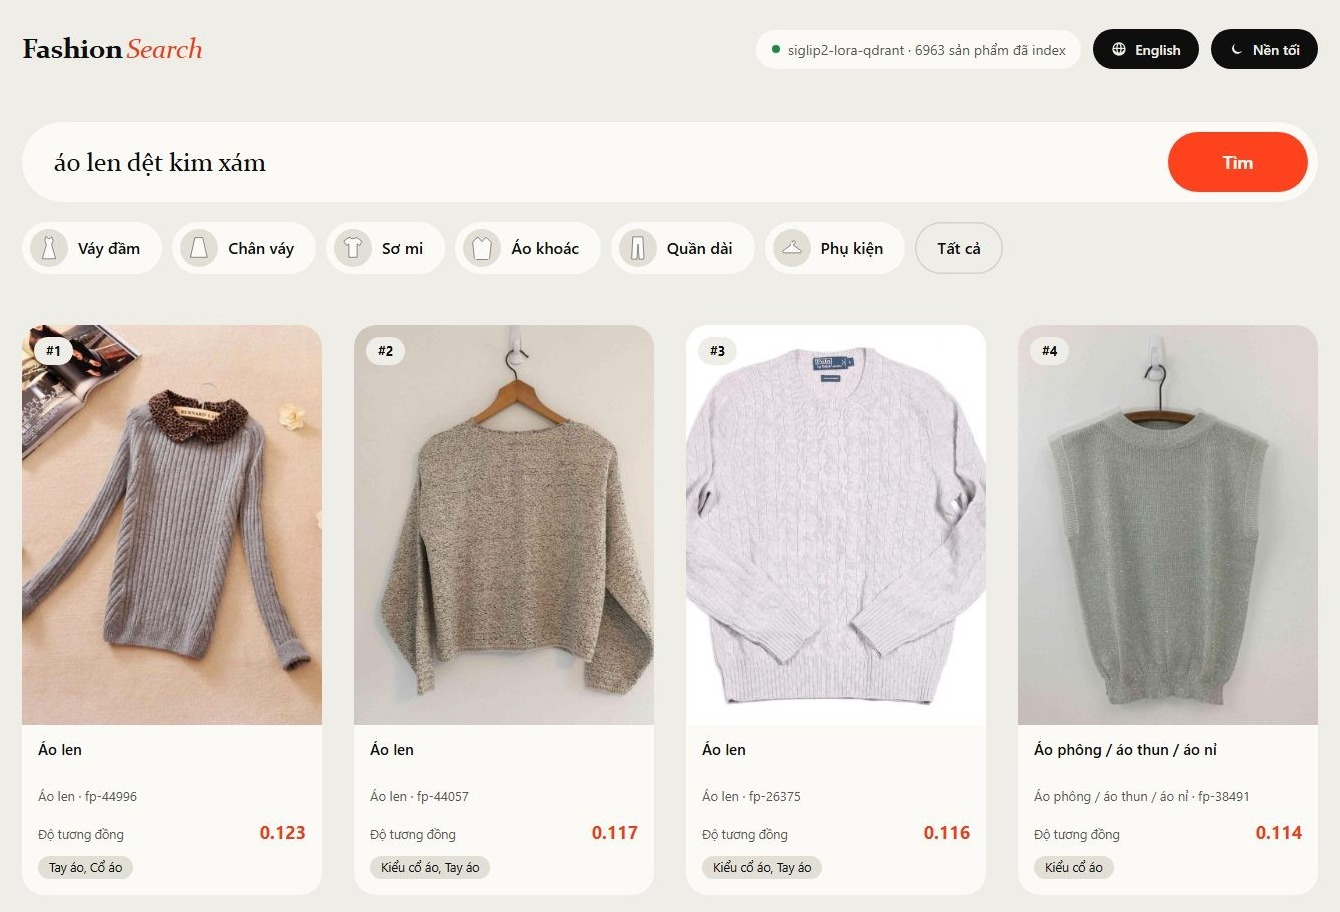
\includegraphics[width=\textwidth]{graphics/ui_ch4_sang_gon.jpg}
\caption{Màn hình tìm kiếm với truy vấn ``áo len dệt kim xám'', đã lược vùng tải ảnh}
\label{fig:c4_ui}
\end{figure}

Giao diện có hai ngôn ngữ (tiếng Việt, tiếng Anh) và hai chế độ màu (nền sáng, nền tối); trình duyệt ghi nhớ lựa chọn cho lần mở sau. Màn hình ban đầu, trước khi tìm, hiện ở cả bốn tổ hợp ngôn ngữ và chế độ màu trên Hình~\ref{fig:c4_home}; ảnh chỉ lấy ô nhập truy vấn, hàng nút chọn nhanh và các ô danh mục, số kết quả, khoá API.

\begin{figure}[H]
\centering
\begin{subfigure}[t]{\textwidth}
\centering
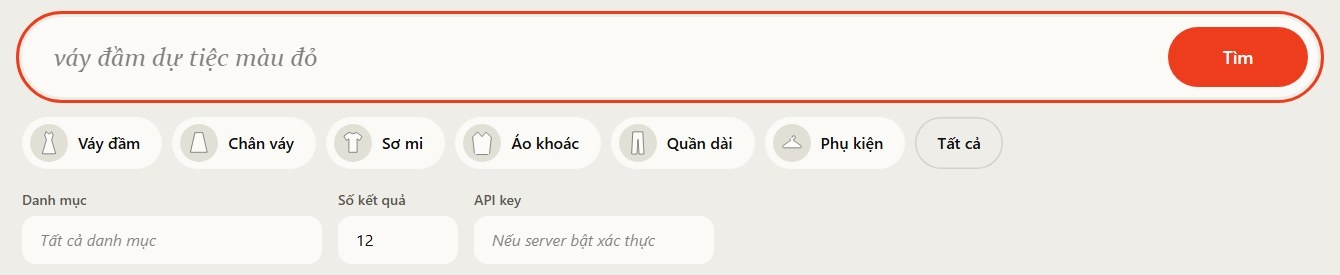
\includegraphics[width=\textwidth]{graphics/home_vi_light_cat.jpg}
\caption{Tiếng Việt, nền sáng}
\end{subfigure}

\vspace{0.4em}
\begin{subfigure}[t]{\textwidth}
\centering
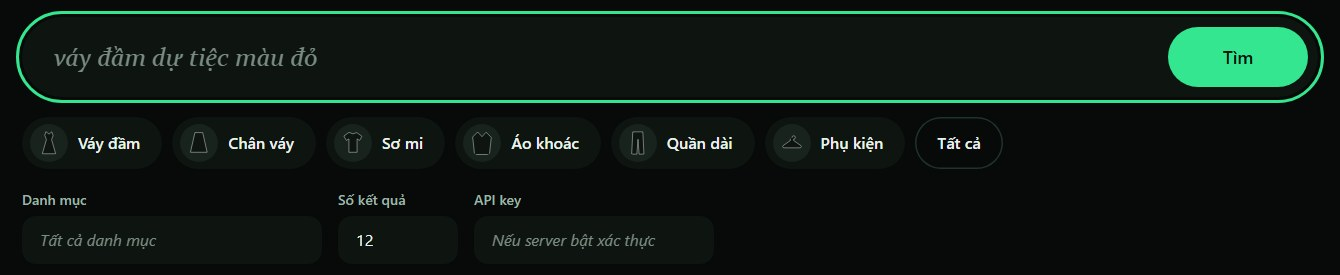
\includegraphics[width=\textwidth]{graphics/home_vi_dark_cat.jpg}
\caption{Tiếng Việt, nền tối}
\end{subfigure}

\vspace{0.4em}
\begin{subfigure}[t]{\textwidth}
\centering
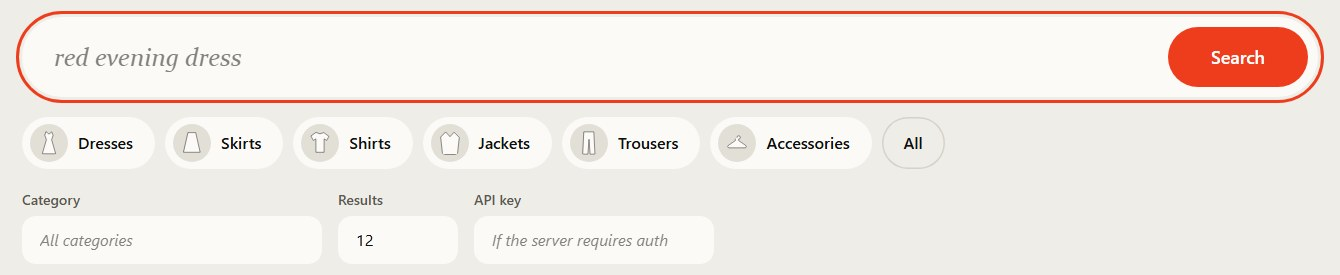
\includegraphics[width=\textwidth]{graphics/home_en_light_cat.jpg}
\caption{Tiếng Anh, nền sáng}
\end{subfigure}

\vspace{0.4em}
\begin{subfigure}[t]{\textwidth}
\centering
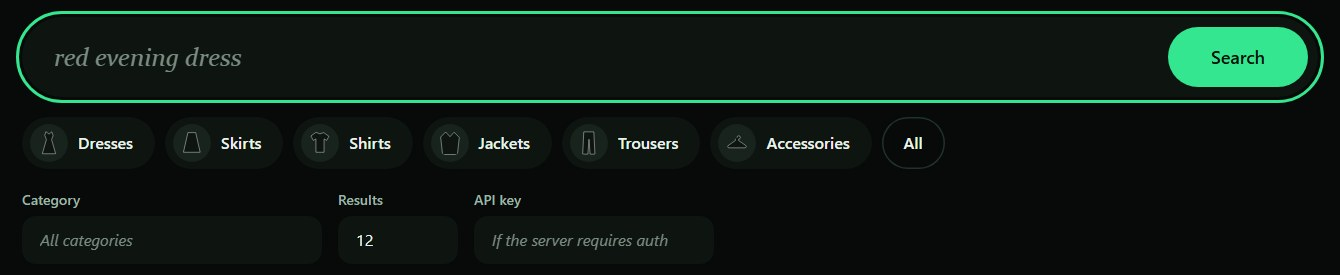
\includegraphics[width=\textwidth]{graphics/home_en_dark_cat.jpg}
\caption{Tiếng Anh, nền tối}
\end{subfigure}
\caption{Ô tìm, hàng nút chọn nhanh và các ô lọc ở màn hình ban đầu, hai ngôn ngữ và hai chế độ màu}
\label{fig:c4_home}
\end{figure}

Toàn bộ màn hình đầu tiên trong cửa sổ rộng được trình bày ở Hình~\ref{fig:c4_full}, với hai cấu hình đại diện (tiếng Việt nền sáng và tiếng Anh nền tối). Phần đầu trang có thanh trạng thái, cho biết bộ tìm kiếm đang chạy và số sản phẩm đã lập chỉ mục, cùng hai nút đổi ngôn ngữ và chế độ màu.

\begin{figure}[H]
\centering
\begin{subfigure}[t]{\textwidth}
\centering
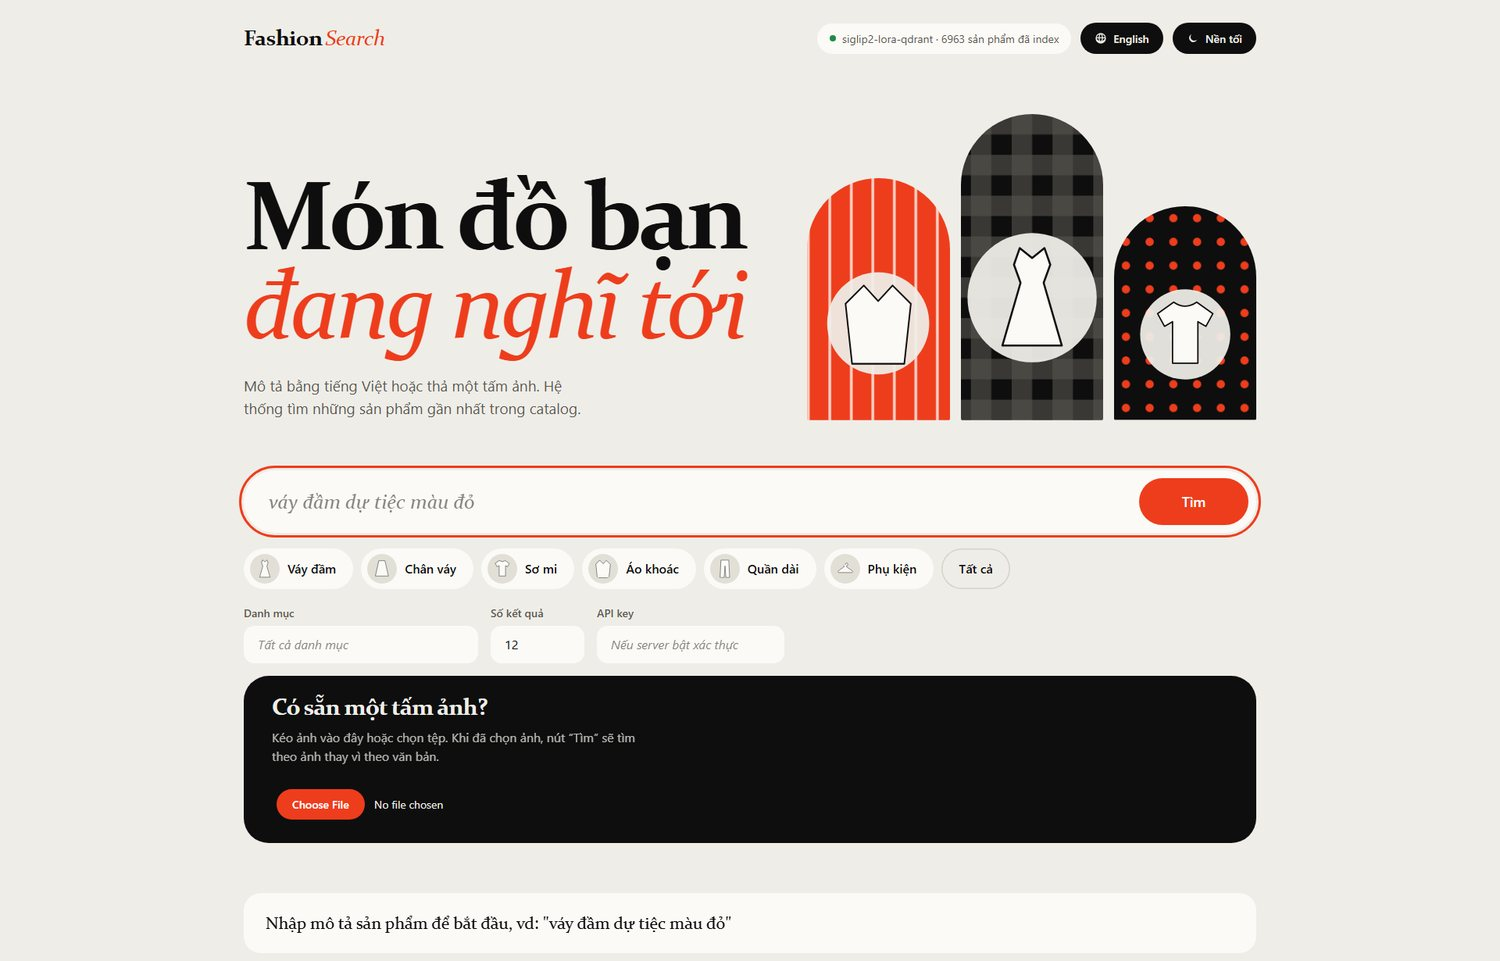
\includegraphics[width=\textwidth]{graphics/full_vi_light_cat.jpg}
\caption{Tiếng Việt, nền sáng}
\end{subfigure}

\vspace{0.6em}
\begin{subfigure}[t]{\textwidth}
\centering
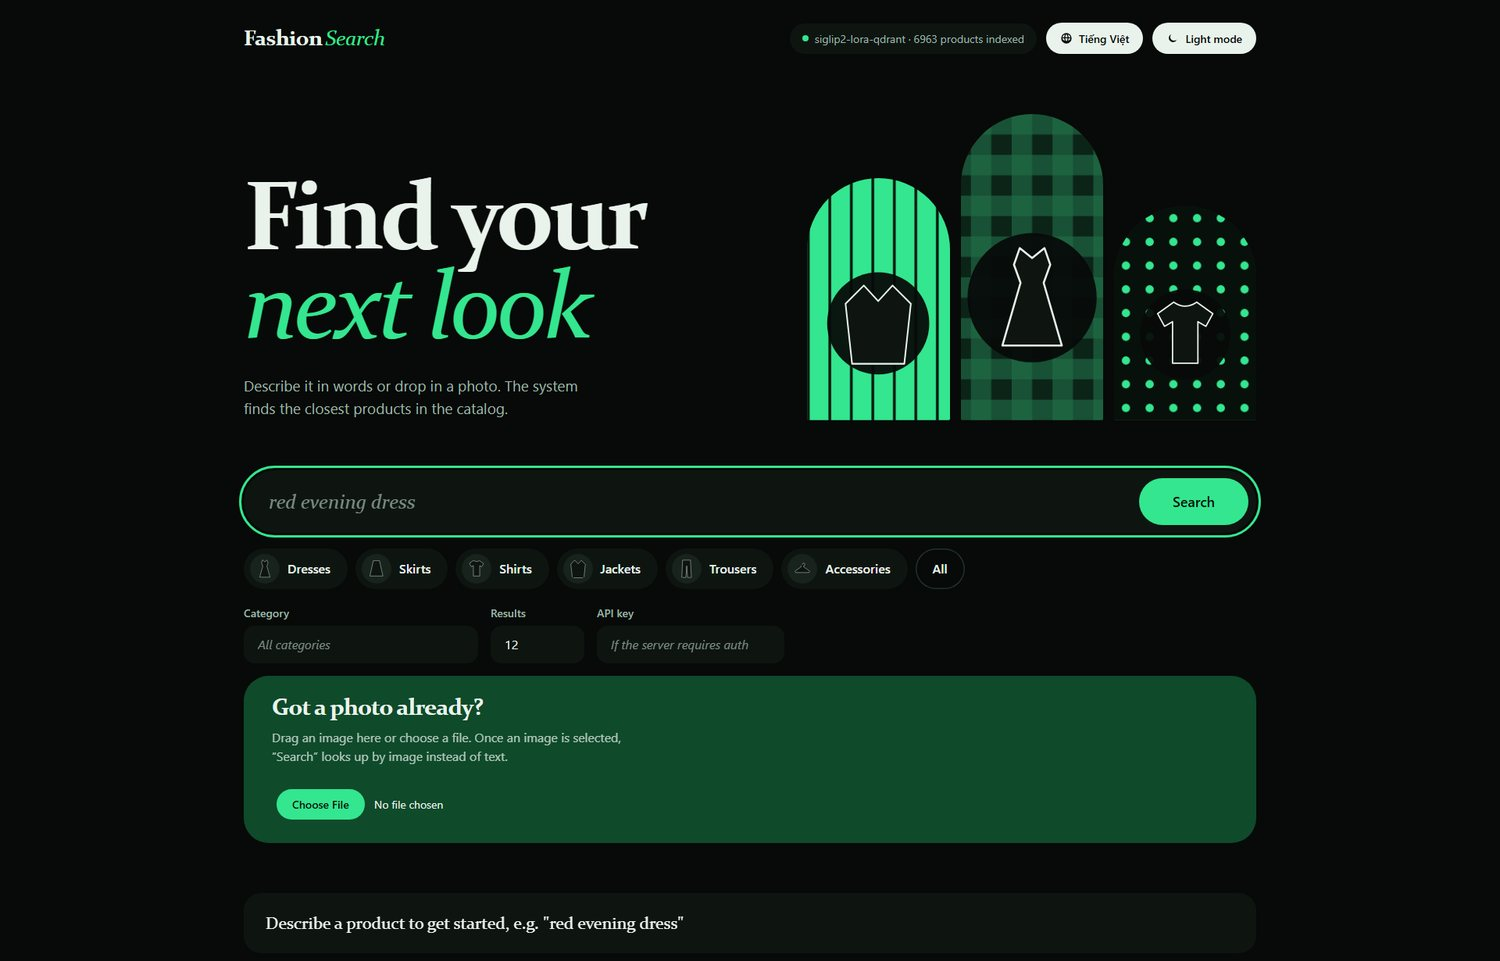
\includegraphics[width=\textwidth]{graphics/full_en_dark_cat.jpg}
\caption{Tiếng Anh, nền tối}
\end{subfigure}
\caption{Màn hình đầu tiên của giao diện web trong cửa sổ rộng, trước khi gửi truy vấn}
\label{fig:c4_full}
\end{figure}

\section{Triển khai và giới hạn}
\label{sec:trien-khai}

\subsection{Triển khai}

Hệ thống chạy trên một máy. Qdrant chạy bằng tệp thực thi gốc phiên bản 1.19.0; tệp mô tả container trong mã nguồn khai báo phiên bản 1.12.4, nên tổ hợp bản container này với máy khách 1.19.0 chưa được thử. Sau khi lập chỉ mục một lần, dịch vụ nạp mô hình rồi nhận truy vấn tại cổng cục bộ.

\subsection{Giới hạn hiện tại}

\begin{itemize}
\item Độ trễ: hệ DoRA chưa đạt chỉ tiêu 200 ms của đề cương trên máy đo (Mục~\ref{sec:danh-gia-dau-ra}).
\item Thực nghiệm: mỗi cấu hình chỉ huấn luyện một lần, với seed 42 (Chương~\ref{chap:danh_gia}).
\item Kiểm thử: bộ kiểm thử tự động gồm 21 tệp với 246 phép kiểm thử, đều đạt ở lần chạy mặc định. Thêm 13 phép kiểm thử cần GPU hoặc Qdrant không nằm trong lần chạy này và chưa được chạy lại trên phiên bản cuối.
\end{itemize}

\subsection{Bảo mật}

Khoá API là tuỳ chọn. Nếu không đặt biến môi trường tương ứng, hai endpoint tìm kiếm mở công khai; nếu đặt, yêu cầu phải mang khoá đúng trong tiêu đề, yêu cầu sai khoá bị từ chối với mã 401. Hệ thống so sánh khoá bằng phép so chuỗi thông thường, nên chưa phòng được tấn công dựa trên thời gian phản hồi.

Endpoint ảnh, trang \texttt{/ui} và trang \texttt{/} công khai theo thiết kế. Endpoint ảnh chặn đường dẫn có thành phần lên thư mục cha, đường dẫn tuyệt đối và tệp không phải ảnh. Cả hai trang hiển thị văn bản từ máy chủ dưới dạng chữ thuần, không chèn mã đánh dấu. Lỗi mất kết nối đến Qdrant trả về mã 503 với thông báo cố định, không lộ địa chỉ hay khoá.

Hệ thống chỉ có xác thực bằng một khoá API tuỳ chọn, chưa có giới hạn tốc độ, TLS, phân quyền theo người dùng hay nhật ký truy cập, nên chỉ chạy cục bộ. Qdrant chạy cục bộ không có khoá. Dữ liệu là bộ Fashionpedia công khai, không chứa dữ liệu cá nhân.
